
\chapter{Numerické metódy}
\label{kap:numeric_methods}

V tejto kapitole si uvedieme numerické metódy zaoberajúce sa hľadaním riešenia rovnice $f(x) = 0$.
Presnejšie majme danú \textit{spojitú funkciu} $f: M \to \mathbb{R}, M \subset \mathbb{R}$. Hľadáme bod
$\bar{x} \in R$ taký, že $f(\bar{x}) = 0$.

Naše numerické metódy túto úlohu riešia len približne, avšak s ľubovoľnou presnosťou.

\section{Newton-Raphsonova metóda}

\textit{Newton-Raphsonova metóda}, známa tiež ako \textit{Newtonova metóda} je iteračná metóda používaná na riešenie
úlohy nášho typu. Snažíme sa skonštruovať postupnosť $\{x_n\}_{n=0}^\infty$ takú, že $x_n \to \bar{x}$.
Podľa Newton-Raphsonovej metódy túto požiadavku spĺňa pustupnosť bodov tvorená nasledovne: 
$$ x_{n+1} = x_n - \frac{f(x_n)}{f'(x_n)}.$$

Na obrázku \ref{obr:newton_raphson} môžeme vidieť ako táto metóda v praxi funguje. Majme zadanú funkciu
$f(x)$ pre ktorú hľadáme jej koreň, teda priesečník s osou $x$. Pre štartovací bod
$x_0$ preložíme bodom $f(x_0)$ dotyčnicu. Ďalšiu iteráciu nájdeme ako priesečník tejto 
dotyčnice s osou $x$. Na obrázku môžeme vidieť štartovací bod $x_0$ a prvé tri iterácie.

\begin{figure}
    \centerline{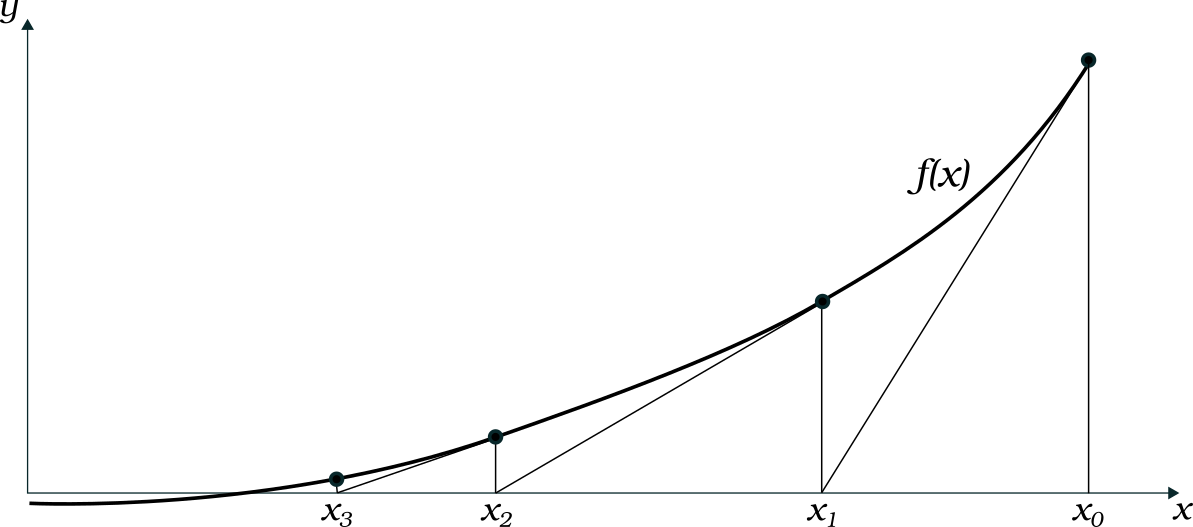
\includegraphics[width=0.8\textwidth]{images/newton_raphson}}
    \caption[Newton-Raphsonova metóda na hľadanie koreňa funckie $f(x)$]{Newton-Raphsonova metóda na hľadanie koreňa funckie $f(x)$}
    %id obrazku, pomocou ktoreho sa budeme na obrazok odvolavat
    \label{obr:newton_raphson}
\end{figure}

Zastavovacích kritérií potrebujeme viacero. Zjavné je ak je $f'(x_n) = 0$ keďže v takomto bode je dotyčnica rovnobežná
s osou $x$, teda by sme nenašli žiadny priesečník. Druhé kritérium je počet iterácií. Tieto 
dva prípady nie sú príliš uspokojivé. Posledné zastavovacie kritérium je v prípade, ak je $f(x_n)$ dostatočne 
malé, teda sme veľmi blízko koreňa. Posledné kritérium sa dá tiež preformulovať na $|x_{n+1} - x_n|$ 
je dostatočne malé.

Nevýhodou Newton-Raphsonovej metódy je to, že potrebujeme poznať derivácie ale aj to, že negarantuje nájdenie
najbližšieho koreňa. Taktiež sa môže stať, že sa táto metóda zacyklí. Príklad takétoho správania môžeme vidieť
na obrázku \ref{obr:cyclic_newton_raphson}.

\begin{figure}
    \centerline{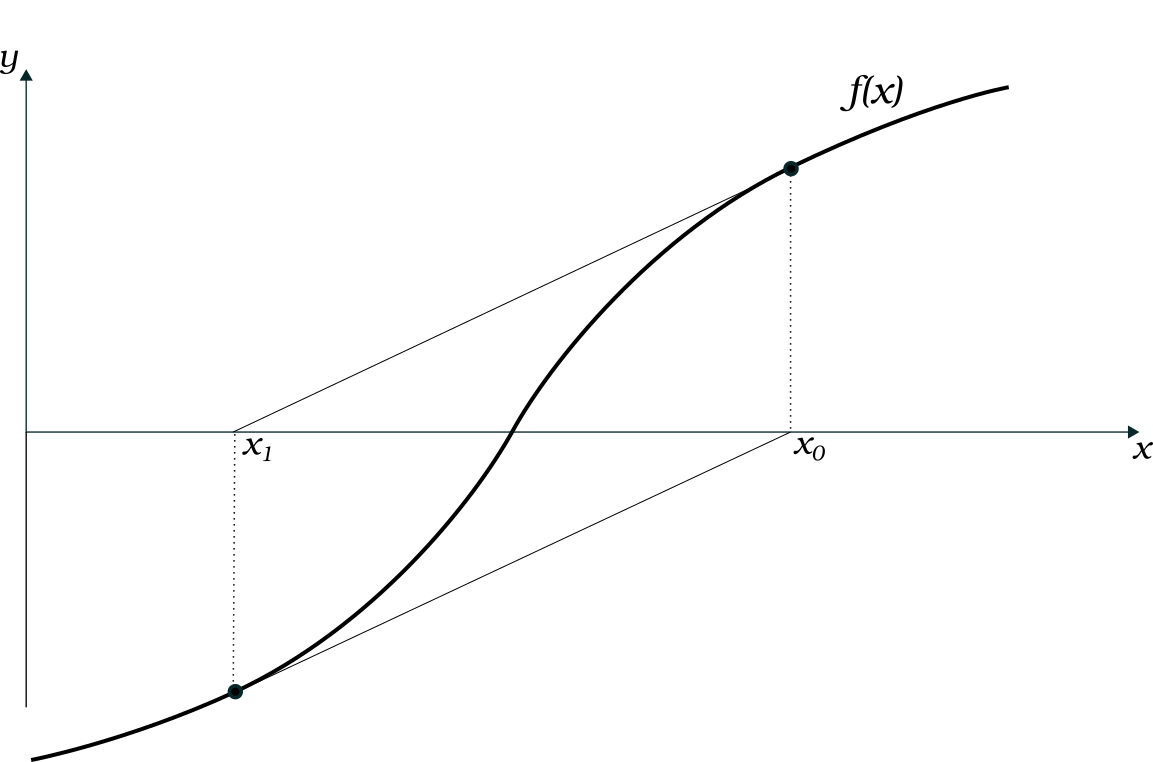
\includegraphics[width=0.8\textwidth]{images/cyclic_newton_raphson}}
    \caption[Zacyklenie Newton-Raphsonovej metódy]{Zacyklenie Newton-Raphsonovej metódy}
    %id obrazku, pomocou ktoreho sa budeme na obrazok odvolavat
    \label{obr:cyclic_newton_raphson}
\end{figure}

\section{Metóda sečníc}

\textit{Metóda sečníc} je akási modifikácia \textit{Newton-Raphsonovej metódy}. 
Môžeme ju použiť napríklad v prípade keď nepoznáme predpis $f'(x)$. 
V tejto metóde dotyčnicu v bode $x_n$ - $f'(x_n)$ nahradíme priamkou 
predchádzajúcou cez body $f(x_n), f(x_{n-1})$ - $\frac{f(x_n) - f(x_{n-1})}{x_n - x_{n-1}}$. 
Túto priamku nazývame \textit{sečnica}. 
Na rozdiel od Newton-Raphsonovej metódy však potrebujeme až $2$ štartovacie body.

Iterácie v metóde sečníc teda vyzerajú nasledovne:
$$ x_{n+1} = x_n - \frac{f(x_n)}{\frac{f(x_n) - f(x_{n-1})}{x_n - x_{n-1}}}.$$

Na obrázku \ref{obr:secant_method} môžeme vidieť vizualizáciu tejto metódy.

\begin{figure}
    \centerline{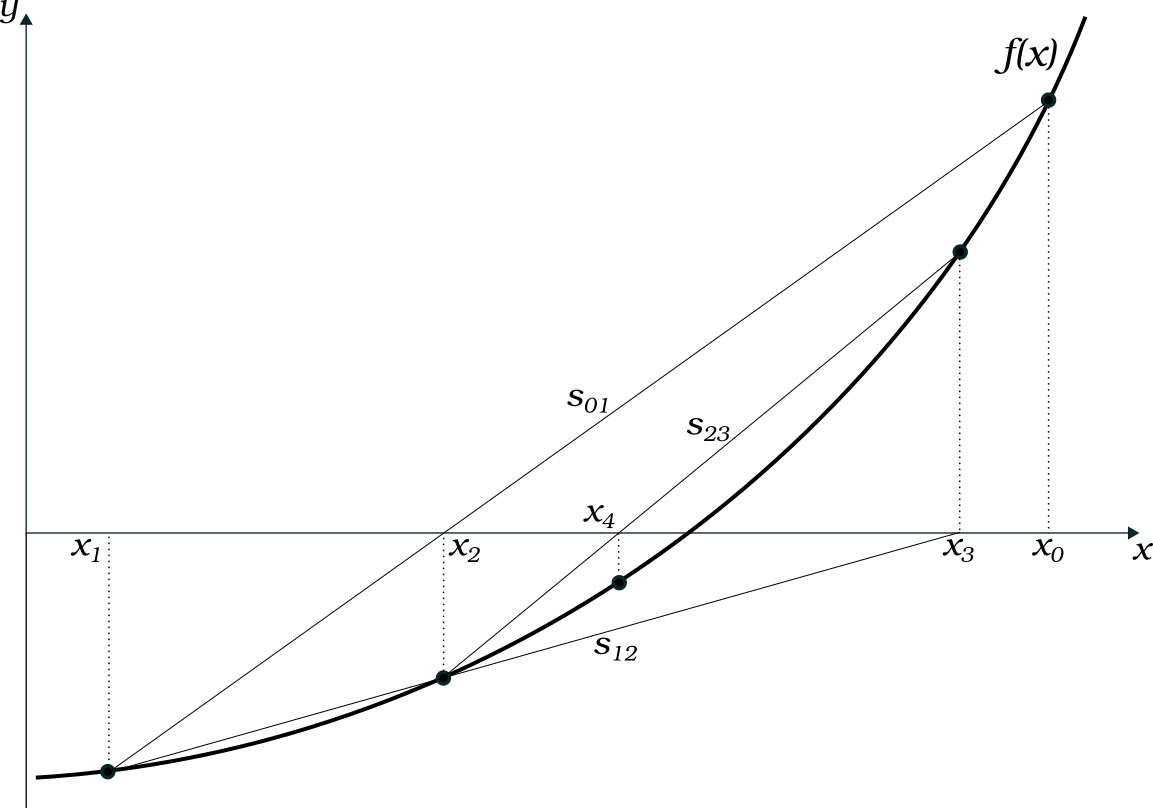
\includegraphics[width=0.8\textwidth]{images/secant_method}}
    \caption[Metóda sečníc na hľadanie koreňa funckie $f(x)$]{Metóda sečníc na hľadanie koreňa funckie $f(x)$}
    %id obrazku, pomocou ktoreho sa budeme na obrazok odvolavat
    \label{obr:secant_method}
\end{figure}

Nevýhodou tejto metódy je, že sa môže tak isto ako Newton-Raphsonova metóda zacykliť, teda 
opäť potrebujeme ako zastavovacie kritérium aj počet iterácii. Taktiež konverguje
pomalšie ako Newton-Raphsonova metóda.

\iffalse
\section{Zjednodušená Newtonova metóda - TODO asi vyhodiť preč}

\textit{Zjednodušená Newtonova metóda} sa môžem použiť v prípade, ak \textit{Newton-Raphsonova metóda} zlyhá na prvom 
zastavovacom kritériu, teda na nulovosti derivácie. Táto metóda nahrádza $f'(x_n)$ dotyčnicou v začiatočnom bode $f'(x_0)$.  
\fi

\section{Metóda bisekcie}

\textit{Metóda bisekcie}, známa tiež ako \textit{Metóda polenia intervalu} je založená 
na pozorovaní, že v okolí koreňa funkčné hodnoty spojitej funnkcie menia znamienko. 
Je to jedna z najpomalších ale zároveň najbezpečnejších metód.

Majme spojitú funkciu $f(x)$ a body $a$ a $b$, také, že $f(a) \cdot f(b) < 0$, teda 
funkčné hodnoty majú v týchto bodoch opačné znamienka. Metóda bisekcie delí tento 
interval na polovicu a na základe znamienka funkčnej hodonty v novom bode $s = (a+b)/2$
rozhodne, či sa koreň nachádza na intervale $(a, s)$ alebo na intervale $(s, b)$. 
Ak platí $f(s) = 0$, potom má funkcia v danom bode koreň. Daný postup sa opakuje, 
pokým nie je splnené niektoré zo zastavovacích kritérií. Na obrázku \ref{obr:bisection}
môžeme vidieť štartovacie body $x_0$ a $x_1$ a tiež prvé 3 iterácie. Vodorovnými
úsečkami so šípkami je znázornená postupná voľba intervalov. 

\begin{figure}
    \centerline{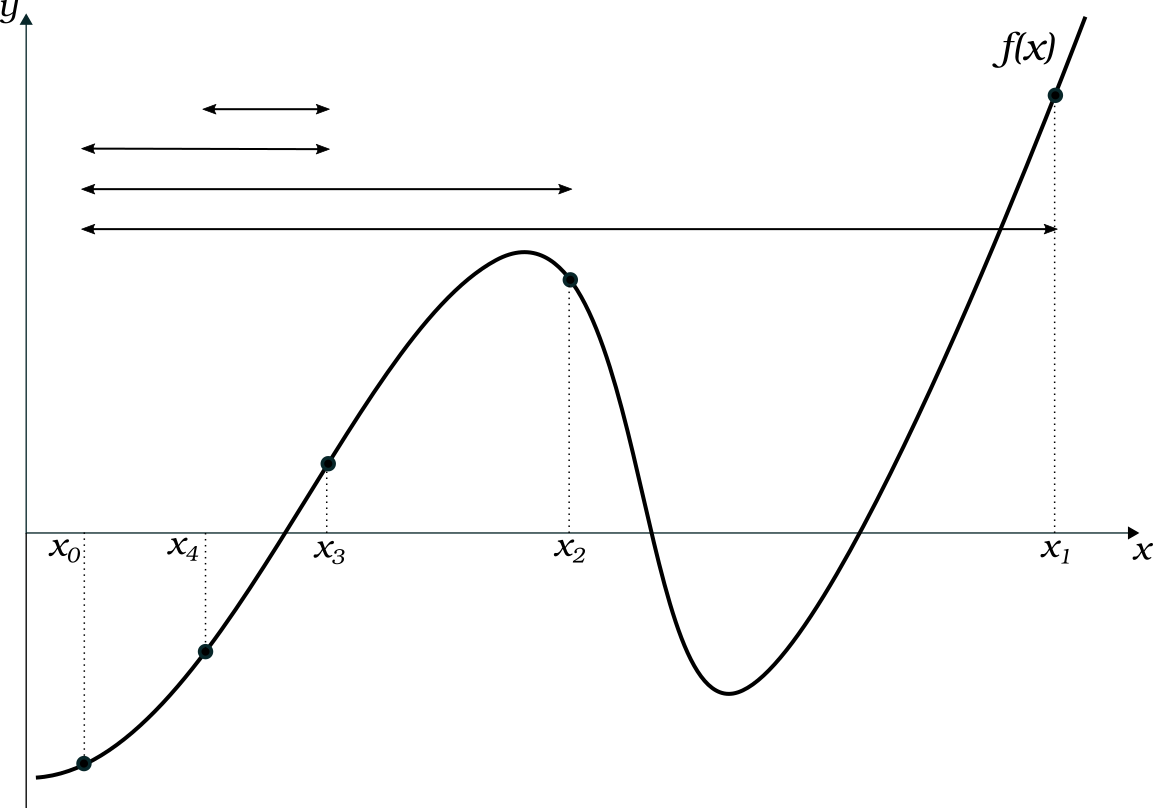
\includegraphics[width=0.8\textwidth]{images/bisection}}
    \caption[Metóda bisekcie na hľadanie koreňa funckie $f(x)$]{Metóda bisekcie na hľadanie koreňa funckie $f(x)$}
    %id obrazku, pomocou ktoreho sa budeme na obrazok odvolavat
    \label{obr:bisection}
\end{figure}

Ak sa na intervale $(a, b)$ nachádza viac koreňov, metóda bisekcie nájde aspoň jeden z nich.

Zjavnou nevýhodou tejto metódy je podmienka štartovacích bodov a taktiež rýchlosť algoritmu. 
Veľkou výhodou však je, že ak vieme, že ne intervale $(a, b)$ sa nachádza práve jeden koreň, 
touto metódou ho nájdeme. \textit{Metóda bisekcie} sa taktiež nemôže zacykliť.

